\section{Assignment 5}
\subsection{Multiple linear regression}
The main task in the first part of the fifths assignment is to find the linear regression of the choosen target over the set of input features.
We have choosen \texttt{num\_hrefs} as a target feature for building linear regression. That is the target feature  in our work is the  number of links that are in the particular article. 

The first thing we did as a preprocessing step for the further analysis was to find all the feautres that seemed to be distributed lognormal and apply to them logarithm transformation.
Example of such a transformation could be seen in the Figures \ref{fig:hist_of_ref_avg_shares}--\ref{fig:hist_log_self_ref_avg_shares}.
 
 
\begin{figure}[h!]
\centering
\begin{minipage}[h]{0.45\linewidth}
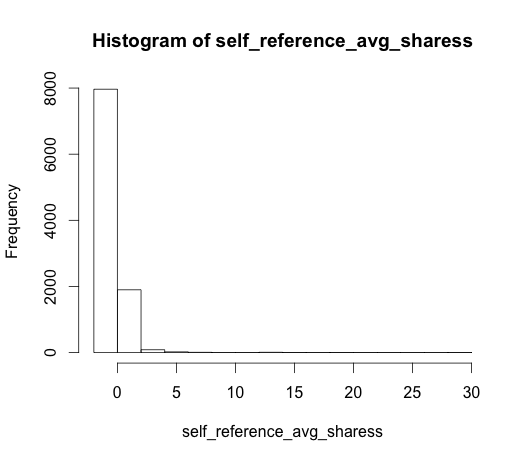
\includegraphics[width=1\linewidth]{images/hist_of_ref_avg_shares}
\caption{Initial distribution of one of the features selected for logarithm transformation.}
\label{fig:hist_of_ref_avg_shares}
\end{minipage}
\hfill
\begin{minipage}[h]{0.45\linewidth}
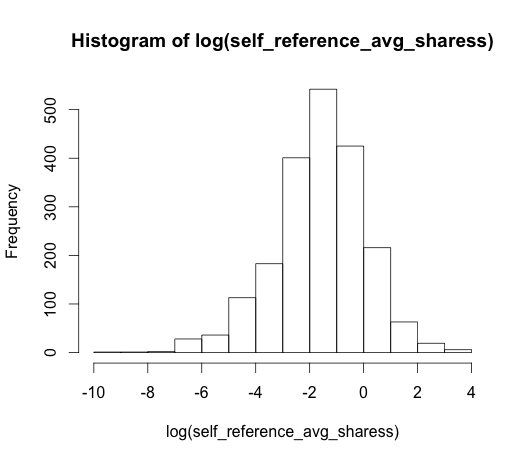
\includegraphics[width=1\linewidth]{images/hist_log_self_ref_avg_shares}
\caption{Distribution of a feature after applying logarithm transformation.}
\label{fig:hist_log_self_ref_avg_shares}
\end{minipage}
\end{figure}

Similarly we have transformed some other features, some of them are: \texttt{num\_hrefs}, \texttt{num\_self\_hrefs}, \texttt{shares}, \texttt{n\_tokens\_content}, \texttt{self\_reference\_avg\_sharess}.


The second step we took was applying the procedure of stepwise regression to find the set of the most influencing independent variables (aka regressors). The code snippet below shows how we have used the bidirectional stepwise regression regarding in the case of raw (unstandartized) data. 

It is worth to mention that we have used the Akaike information criterion for selection the proper number of explanatory variables and the proper values of coefficients in linear regression model.

\begin{knitrout}
\definecolor{shadecolor}{rgb}{0.969, 0.969, 0.969}\color{fgcolor}\begin{kframe}
\begin{alltt}
\hlstd{min.model} \hlkwb{<-} \hlkwd{lm}\hlstd{(num_hrefs} ~ \hlnum{1}\hlstd{,} \hlkwc{data}\hlstd{= data}\hlstd{)}
\hlstd{max.model} \hlkwb{<-} \hlkwd{lm}\hlstd{(num_hrefs} ~\hlstd{.,} \hlkwc{data} = data\hlstd{)}
\hlstd{bidir.model} \hlkwb{<-} \hlkwd{step}\hlstd{(min.model,}  \hlkwc{scope} \hlstd{=} list(upper=max.model)\hlstd{,} 
		\hlkwc{data} = data, \hlkwc{direction} = "both", \hlkwc{trace} = \hlnum{0}\hlstd{)}
\hlkwd{summary}\hlstd{(bidir.model))}
## Call:
## lm(formula = num_hrefs ~ n_tokens_content + num_self_hrefs + 
##     n_unique_tokens + num_keywords + num_imgs + timedelta + data_channel_is_socmed + 
##     weekday_is_sunday + average_token_length + avg_negative_polarity + 
##     global_sentiment_polarity + title_sentiment_polarity, data = data)
## 
## Residuals:
##     Min      1Q  Median      3Q     Max 
## -3913.8   -14.1     2.4    22.6   210.7 
## 
## Coefficients:
##                             Estimate Std. Error t value Pr(>|t|)    
## (Intercept)               -4.477e+01  3.981e+01  -1.125 0.260700    
## n_tokens_content           9.672e-01  1.043e-02  92.718  < 2e-16 ***
## num_self_hrefs             3.122e-02  1.791e-03  17.431  < 2e-16 ***
## n_unique_tokens           -1.786e+02  2.336e+01  -7.646 2.27e-14 ***
## num_keywords               5.126e+00  1.149e+00   4.463 8.18e-06 ***
## num_imgs                  -1.052e+00  2.824e-01  -3.726 0.000196 ***
## timedelta                  4.165e-02  1.049e-02   3.972 7.19e-05 ***
## data_channel_is_socmed    -3.248e+01  9.215e+00  -3.525 0.000425 ***
## weekday_is_sunday         -2.421e+01  8.329e+00  -2.906 0.003664 ** 
## average_token_length       1.734e+01  7.884e+00   2.200 0.027858 *  
## avg_negative_polarity     -3.797e+01  1.906e+01  -1.992 0.046349 *  
## global_sentiment_polarity  4.546e+01  2.524e+01   1.801 0.071707 .  
## title_sentiment_polarity  -1.255e+01  8.165e+00  -1.537 0.124417    
## ---
## Signif. codes:  0 ‘***’ 0.001 ‘**’ 0.01 ‘*’ 0.05 ‘.’ 0.1 ‘ ’ 1
## 
## Residual standard error: 214.9 on 9987 degrees of freedom
## Multiple R-squared:  0.9044,	Adjusted R-squared:  0.9043 
## F-statistic:  7877 on 12 and 9987 DF,  p-value: < 2.2e-16
\end{alltt}
\end{kframe}
\end{knitrout}

To obtain the standardized data we define the function \texttt{normalize} as the subtraction from each element of a vector its mid-range and normalizing this difference by half-range of the possible values in that vector. The multiple linear regression results over standardized features,  which were chosen in the same manner as was described before -- by the bidirectional stepwise regression using  Akaike information, regarding to standardized dependent feature \texttt{num\_hrefs} is shown in the code snippet below. 
\begin{knitrout}
\definecolor{shadecolor}{rgb}{0.969, 0.969, 0.969}\color{fgcolor}\begin{kframe}
\begin{alltt}
## data.nlm - standardized data
\hlstd{data.nrm} \hlkwb{<-} \hlkwd{as.data.frame}(\hlkwd{apply}(data, \hlkwc{MARGIN} = \hlnum{2}, normalize))

\hlstd{min.model.nrm} \hlkwb{<-} \hlkwd{lm}(num_hrefs~\hlnum{1}, \hlkwc{data} =data.nrm)
\hlstd{max.model.nrm} \hlkwb{<-} \hlkwd{lm}(num_hrefs~., \hlkwc{data}=data.nrm)
\hlstd{bidir.model.nrm} \hlkwb{<-} \hlkwd{step}(min.model.nrm,  \hlkwc{scope} = list(upper=max.model.nrm), 
\hlkwc{data} = data.nrm, \hlkwc{direction} = "both", \hlkwc{trace} = \hlnum{0})
\hlkwd{summary}\hlstd{(bidir.model.nrm))}
## Call:
## lm(formula = num_hrefs ~ n_tokens_content + num_self_hrefs + 
##     n_unique_tokens + num_keywords + num_imgs + timedelta + data_channel_is_socmed + 
##     weekday_is_sunday + average_token_length + avg_negative_polarity + 
##     global_sentiment_polarity + title_sentiment_polarity, data = data.nrm)
## 
## Residuals:
##      Min       1Q   Median       3Q      Max 
## -1.95444 -0.00706  0.00120  0.01128  0.10521 
## 
## Coefficients:
##                            Estimate Std. Error t value Pr(>|t|)    
## (Intercept)               -0.045000   0.011792  -3.816 0.000136 ***
## n_tokens_content           0.968096   0.010441  92.718  < 2e-16 ***
## num_self_hrefs             0.031221   0.001791  17.431  < 2e-16 ***
## n_unique_tokens           -0.043680   0.005713  -7.646 2.27e-14 ***
## num_keywords               0.011519   0.002581   4.463 8.18e-06 ***
## num_imgs                  -0.033631   0.009027  -3.726 0.000196 ***
## timedelta                  0.007519   0.001893   3.972 7.19e-05 ***
## data_channel_is_socmed    -0.008111   0.002301  -3.525 0.000425 ***
## weekday_is_sunday         -0.006044   0.002080  -2.906 0.003664 ** 
## average_token_length       0.031257   0.014210   2.200 0.027858 *  
## avg_negative_polarity     -0.009482   0.004759  -1.992 0.046349 *  
## global_sentiment_polarity  0.012577   0.006983   1.801 0.071707 .  
## title_sentiment_polarity  -0.006265   0.004077  -1.537 0.124417    
## ---
## Signif. codes:  0 ‘***’ 0.001 ‘**’ 0.01 ‘*’ 0.05 ‘.’ 0.1 ‘ ’ 1
## 
## Residual standard error: 0.1073 on 9987 degrees of freedom
## Multiple R-squared:  0.9044,	Adjusted R-squared:  0.9043 
## F-statistic:  7877 on 12 and 9987 DF,  p-value: < 2.2e-16
\end{alltt}
\end{kframe}
\end{knitrout}

Comparing two outputs it is easy to see that nothing has changed except the absolute values of regression parameter  coefficients.
Particularly, we can see that in both cases the most influencing features, $R^2$ and F-statistic are the same.  This can be explained by the procedure of standardization: it changes the scale of features, but all of the relations between them remain the same.  Here we can also highligh the fact that determinacy coefficient is an with respect to feautre scaling.

\subsection{Bootstrap for determinacy coefficient}
The determinacy coefficients $R^2$ and adjusted $R^2$ of the multiple linear regression described above  are equal to $0.9044$ and $0.9043$ respectively. 

To estimate the 95\%  confidence interval of determinacy coefficient (adjusted) we have performed  the bootstrap  with 5000 trials. The resultant histogram is represented in Figure \ref{fig:hist_r_squared_bootstrap_assign5}. 

\begin{figure}[h!]
 \begin{center}
    \center 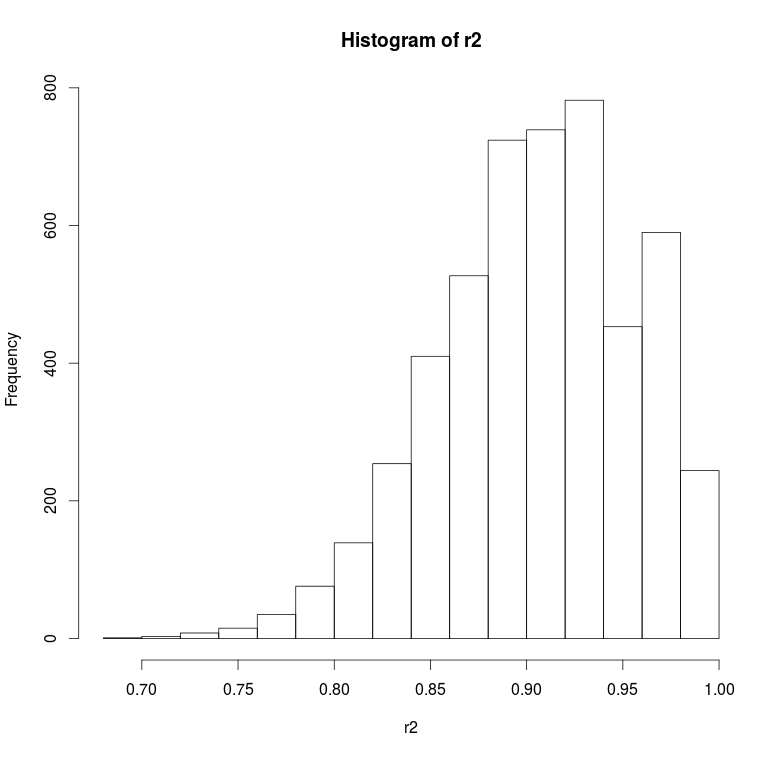
\includegraphics[width = 0.7\textwidth]{hist_r_squared_assign5.png}
   \caption{Histogram of adjusted determinacy coefficients $R^2$ in multiple linear regression with target feature \texttt{$\log$(num\_hrefs)}}
   \label{fig:hist_r_squared_bootstrap_assign5}
 \end{center}
\end{figure} 

From the histogram one could see that the distribution is unlikely to be similar to normal (p-value is equal to $ 1.487\cdot 10^{-10} $ according to Shapiro-Wilk test of normality), therefore we compute non-pivotal confidence interval for $R^2$:
\begin{knitrout}
\definecolor{shadecolor}{rgb}{0.969, 0.969, 0.969}\color{fgcolor}\begin{kframe}
\begin{alltt}
alpha \hlkwb{<-} \hlnum{0.95} # Confidence level
# r2 --- sample of adjusted determinacy coefficients
CI_R2 \hlkwb{<-} \hlkwd{c}\hlstd{(}\hlkwd{quantile}\hlstd{(r2, }\hlkwc{probs}\hlstd{ = (}\hlnum{1} \hlopt{-} alpha)\hlopt{/}\hlnum{2}), 
           \hlkwd{quantile}\hlstd{(r2, }\hlkwc{probs} \hlstd{= (}\hlnum{1} \hlopt{+} alpha)\hlopt{/}\hlnum{1}))
##      2.5%     97.5% 
## 0.7975380 0.9999989 
\end{alltt}
\end{kframe}
\end{knitrout}

The determinacy coefficient from initial model $R^2_{adj} = 0.9043$ is closer to the right border, but lies within the interval. 


\subsection{Linear and Fisher discriminant rules}
In the third part of the fifths assignment one should divide the dataset into two groups, apply to both of them each of the discriminant rules (Linear, Fisher) and measure  accuracy of each of the models with the cross-validation techinque.

So the first we had to do was to meaningfully choose the criterion by which to split our data in two parts. 
To accomplish this task we have performed SVD decomposition and have figured out what feauture indexies  correspond to the most distant values of components of right eigenvector. As one can see in the Figures \ref{fig:svd_for_pca}--\ref{fig:svd_eigenvector} the most outstanding features in the first vector (which in turn corresponds to the most <<important>> first eigenvalue) are features with indexies 25, 26, 27, 28, 29. 

That are the features with the following short titles: 

 \texttt{global\_sentiment\_polarity},
 
 
 \texttt{global\_rate\_positive\_words},
 
 
 \texttt{global\_rate\_negative\_words},
  \texttt{rate\_positive\_words},
   \texttt{rate\_negative\_words}.    

So we define a new feauture as a linear combinations of the features mentioned above and call it \texttt{label}. Obviously, this feature is about the mood of the article. We have also figured out that there are three types of sentiment each of the article posesses: positive, negative and mixed/undefined.




\begin{figure}[h!]
\centering
\begin{minipage}[h]{0.45\linewidth}
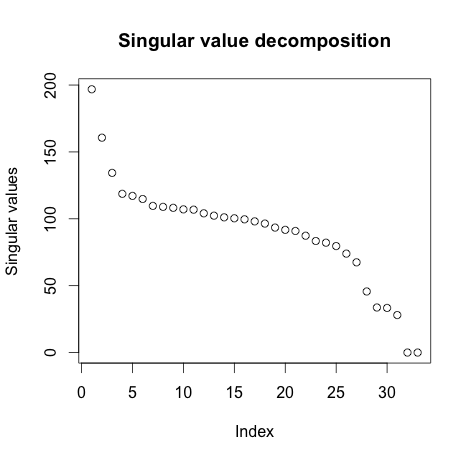
\includegraphics[width=1\linewidth]{images/svd_for_pca}
\caption{Singular values of a data matrix according to the SVD decomposition}
\label{fig:svd_for_pca}
\end{minipage}
\hfill
\begin{minipage}[h]{0.45\linewidth}
	\centering
	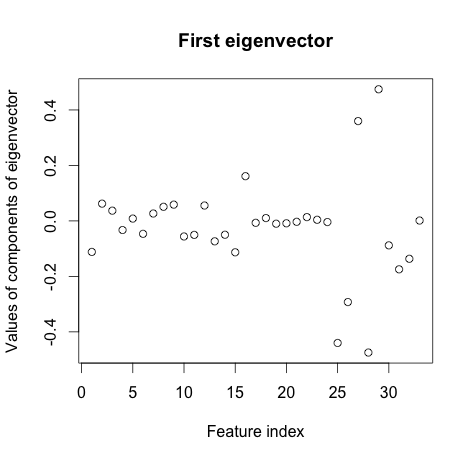
\includegraphics[width=1.00\linewidth]{images/svd_eigenvector}
	\caption{Values of first right singular vector}
	\label{fig:svd_eigenvector}
\end{minipage}
\end{figure}


The best we can do to visualize this mood feature is to perfrom PCA projections on the 2d plane, which is presented in Figures \ref{fig:pca_projection_plot}--\ref{fig:pca_without_mixed}. 

 


\begin{figure}[h!]
	\centering
	\begin{minipage}[h]{0.45\linewidth}
	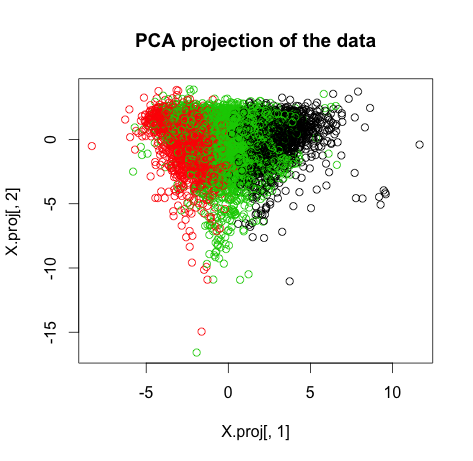
\includegraphics[width=1.1\linewidth]{images/pca_projection_plot}
	\caption{Black circles corresponds to negative articles, red -- to the positive ones and green are associated with those, which are of the mixed mood.}
	\label{fig:pca_projection_plot}
	\end{minipage} 
	\hfill
	\begin{minipage}[h]{0.45\linewidth}
	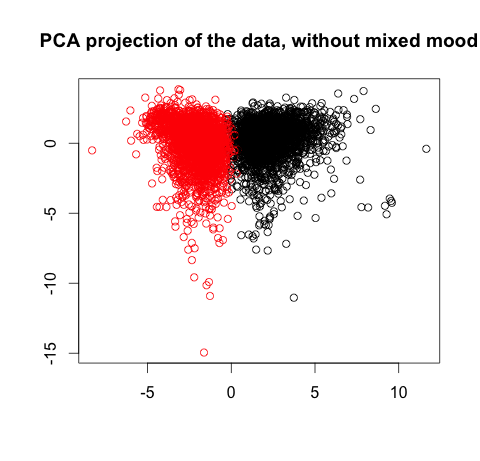
\includegraphics[width=1.1\linewidth]{images/pca_without_mixed}
	\caption{PCA projection without neutral/mixed mood articles}
	\label{fig:pca_without_mixed}
	\end{minipage}
\end{figure}

After determining the splitting feature  we train two different algorithms  (Fisher / Linear discriminant rule) on the part of the data which is allocated by $2$- and  $10$-fold cross-validation techiques. 


\begin{table}[h]
\centering
\label{tbl:fish_lin_disc}
\caption{Fisher versus Linear Discriminant error rate}
\begin{tabular}{|c|c|c|}
	\hline  & Mean error with 2-folds & Mean error with 10-folds \\ 
	\hline Linear Discriminant & 0.005575021  &  0.005342917 \\ 
	\hline Fisher Discriminant  & 0.005110445   & 0.004645782  \\ 
	\hline 
\end{tabular} 
\end{table} 

The result we get is rather easy to explain. It is obvious that Fisher Discriminant Rule (FDR) is better no matter of what $ k $-fold is used. 

From the theory we know that LDR has several assumptions of condition expectaions being distributed  normally. 

FDR doesn't have such a assumption but in case theese probabilities are in fact normal, FDR and LDR are absolutely equal. So FDR is not at least worse than LDR. 

For code and further details of implementation one could see attachements. 





